\section{Function Oriented}

Object-oriented design is the process of planning a system of interacting objects for the purpose of solving a software problem. It is one approach to software design. An object contains encapsulated data and procedures grouped together to represent an entity. The 'object interface' defines how the object can be interacted with. An object-oriented program is described by the interaction of these objects. Object-oriented design is the discipline of defining the objects and their interactions to solve a problem that was identified and documented during object-oriented analysis.

\iffalse
 basic requirement of this app is that the user must be having ANDROID
Operating System in his phone or tablet. The minimum version of Androids Operating
System must be ICECREAM SANDWICH. All the versions of Android OS above
IcecreamSandwich( i.e. Jellybean, Kitkat, Lollipop,Marshmallows) will support this
app. A user needs Monitary app installed in device .


\noindent As shown in the Figure \ref{fig:1}, .\\Brief introduction showing the features available in the application.

\begin{figure}[ht]
\centering
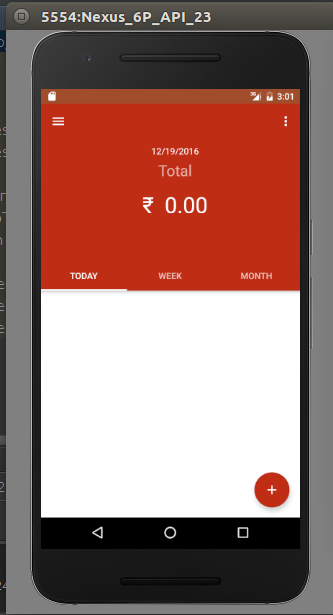
\includegraphics[scale=0.5]{images/s1.png}
\caption{Screen 1}
\label{fig:1}
\end{figure}

\noindent This are the options the navigation drawer the app will contain. These will contain the screens the user can navigate too that can be seen in Figure \ref{fig:2}. \\

\begin{figure}[ht]
	\centering
	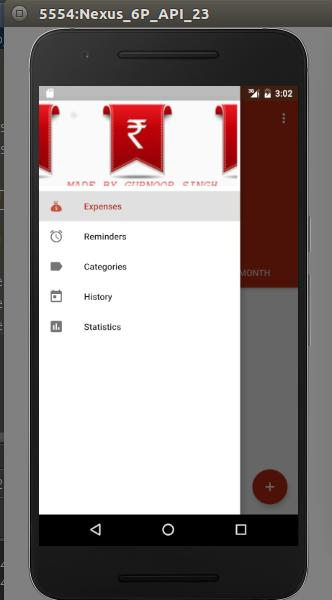
\includegraphics[scale=0.49]{images/s2.png}
	\caption{Screen 2}
	\label{fig:2}
\end{figure}

\noindent  Statistics will be able to change according to the dates selected. Default values will be the current week. User Will be able to see diagrams according to Quantity and
days, Quantity and categories and others.as seen in the Figure \ref{fig:3}.\\

\begin{figure}[ht]
\centering
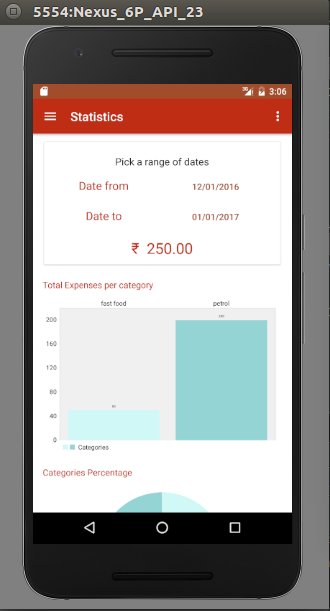
\includegraphics[scale=0.5]{images/s3.png}
\caption{Screen 3}
\label{fig:3}
\end{figure}

\noindent Reminder view will contain details from the reminder created and the user can edit
the reminder values. in Figure \ref{fig:4}. \\

\begin{figure}[ht]
\centering
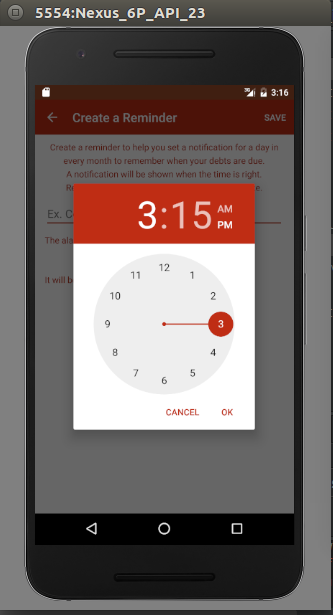
\includegraphics[scale=0.38]{images/s4.png}
\caption{Screen 4}
\label{fig:4}
\end{figure}

\noindent Reminder screen will show the current saved Reminder and if they are active or not.
To activate one it will have a switch next to the name so it can be activated in any
moment. The user will be able to erase and add from this view as seen in the Figure \ref{fig:5}. It's named as output.dxf. We can open that file in LibreCAD directly from the command-line.\\


\begin{figure}[ht]
\centering
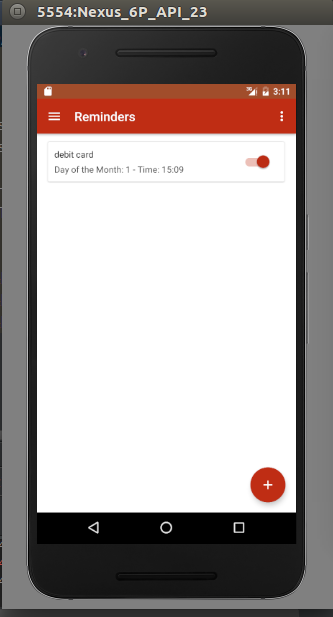
\includegraphics[scale=0.5]{images/s6.png}
\caption{Screen 5}
\label{fig:5}
\end{figure}

\noindent Expenses View is the main screen that will be showed. The user will be able to add expenses and see a total amount in Today, Week and Month. as shown in Figure \ref{fig:6}. 

\begin{figure}[ht]
\centering
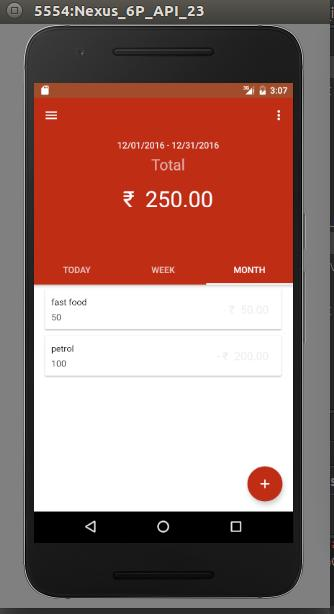
\includegraphics[scale=0.38]{images/s61.png}
\caption{Screen 6}
\label{fig:6}
\end{figure}

\noindent This activity will provide necessary help to the user. One can also mail the maker
(GURNOOR SINGH) for further queries as shown in Figure \ref{fig:7}. 

\begin{figure}[ht]
\centering
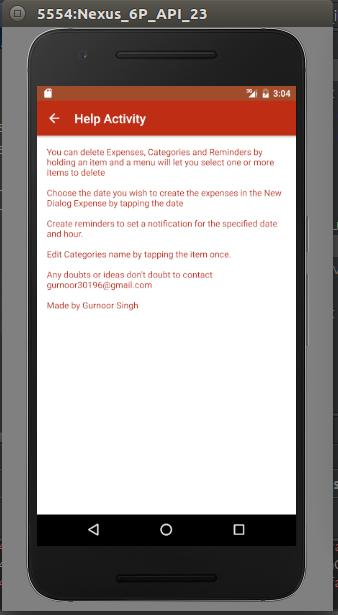
\includegraphics[scale=0.38]{images/s7.png}
\caption{Screen 7}
\label{fig:7}
\end{figure}
\noindent User will be able to add and delete categories from the Categories View \ref{fig:8}. 

\begin{figure}[ht]
\centering
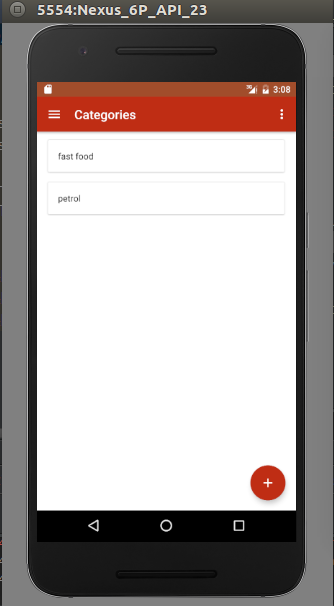
\includegraphics[scale=0.38]{images/s8.png}
\caption{Screen 8}
\label{fig:8}
\end{figure}
\fi

\section{Detail Design}
The design phase involves converting the informational, functional, and network requirements identified during the initiation and planning phases into unified design specifications that developers use to script programs during the development phase. Program designs are constructed in various ways. Using a top-down approach, designers first identify and link major program components and interfaces, then expand design layouts as they identify and link smaller subsystems and connections. Using a bottom-up approach, designers first identify and link minor program components and interfaces, then expand design layouts as they identify and link larger systems and connections.
 
Contemporary design techniques often use prototyping tools that build mock-up designs of items such as application screens, database layouts, and system architectures. End users, designers, developers, database managers, and network administrators should review and refine the prototyped designs in an iterative process until they agree on an acceptable design.
Designers should carefully document completed designs. Detailed documentation enhances a programmer’s ability to develop programs and modify them after they are placed in production. The documentation also helps management ensure final programs are consistent with original goals and specifications. Organizations should create initial testing, conversion, implementation, and training plans during the design phase. Additionally, they should draft user, operator, and maintenance manuals.

For design of the website project:
\begin{itemize}
	\item First Database has to be designed which can be used to handle all the requirements of the users.
	\item The basic structure of the website has to be designed.  
	\item The main template to be used for the website is designed.
\end{itemize}

\section{Data Flow Diagram}
Information moves through software, it is modified by a series of transformations. Data flow diagram is a graphical representation that depicts information flow and the transforms that are applied as data move from input to output. The basic form of a data flow diagram, also known as a data flow graph or a bubble chart.
The data flow diagram may be used to represent a system or software at any level of abstraction. DFDs may be partitioned into levels that represent increasing information flow and functional detail. The DFD provides a mechanism for functional modeling as well as information flow modeling.
\begin{figure}[ht]
\centering
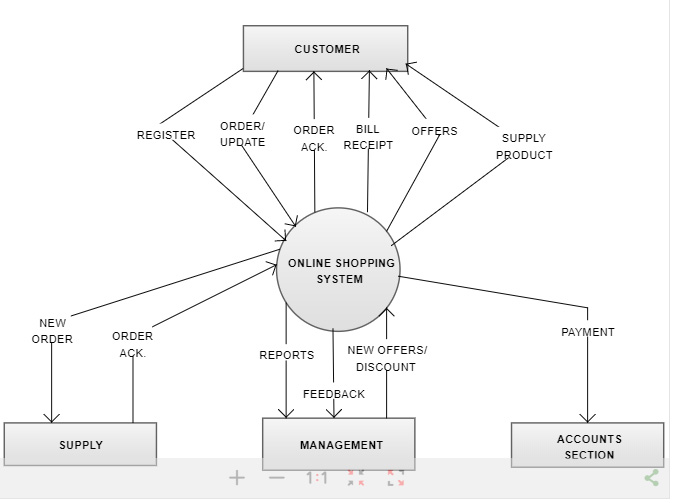
\includegraphics[scale=0.40]{images/pil.png}
\caption{Data Flow Diagram}
\end{figure}

\section{Database Design}
\subsection{ER Diagrams}
An entity-relationship (ER) diagram, a graphical representation of entities and their relationships to each other, typically used in computing in regard to the organization of data within databases or information systems. An entity is a piece of data-an object or concept about which data is stored. A relationship is how the data is shared between entities.
Entities may be characterized not only by relationships, but also by additional properties (attributes), which include identifiers called "primary keys". Diagrams created to represent attributes as well as entities and relationships may be called entity-attribute-relationship diagrams, rather than entity-relationship models.
There is a tradition for ER/data models to be built at two or three levels of abstraction. Note that the conceptual-logical-physical hierarchy below is used in other kinds of specification, and is different from the three schema approach to software engineering.
\subsection{Normalization}
Database Normalisation is a technique of organizing the data in the database. Normalization is a systematic approach of decomposing tables to eliminate data redundancy and undesirable characteristics like Insertion, Update and Deletion Anamolies. It is a multi-step process that puts data into tabular form by removing duplicated data from the relation tables.
Normalization is used for mainly two purpose:

\begin{itemize}
	\item Eliminating reduntant(useless) data.
	\item Ensuring data dependencies make sense i.e data is logically stored.  
\end{itemize}
Normalization rule are divided into following normal form.
\subsection{First Normal Form(1NF)}
As per First Normal Form, no two Rows of data must contain repeating group of information i.e each set of column must have a unique value, such that multiple columns cannot be used to fetch the same row. Each table should be organized into rows, and each row should have a primary key that distinguishes it as unique.

The Primary key is usually a single column, but sometimes more than one column can be combined to create a single primary key.
\subsection{Second Normal Form(2NF)}
As per the Second Normal Form there must not be any partial dependency of any column on primary key. It means that for a table that has concatenated primary key, each column in the table that is not part of the primary key must depend upon the entire concatenated key for its existence. If any column depends only on one part of the concatenated key, then the table fails Second normal form.
\subsection{Third Normal Form(3NF}
Third Normal form applies that every non-prime attribute of table must be dependent on primary key, or we can say that, there should not be the case that a non-prime attribute is determined by another non-prime attribute. So this transitive functional dependency should be removed from the table and also the table must be in Second Normal form.
\subsection{Boyce and Codd Normal Form (BCNF)}
Boyce and Codd Normal Form is a higher version of the Third Normal form. This form deals with certain type of anomaly that is not handled by 3NF. A 3NF table which does not have multiple overlapping candidate keys is said to be in BCNF. For a table to be in BCNF, following conditions must be satisfied:
\begin{itemize}
	\item R must be in 3rd Normal Form
	\item and, for each functional dependency ( X → Y ), X should be a super Key. 
\end{itemize}
\subsection{Database Manipulation}
Data manipulation is the process of changing data in an effort to make it easier to read or be more organized. For example, a log of data could be organized in alphabetical order, making individual entries easier to locate. Data manipulation is often used on web server logs to allow a website owner to view their most popular pages as well as their traffic sources.

Users in the Accounting field or other fields that work with numbers often manipulate data to figure out costs of products, trends in sales, potential tax obligations, or how well merchandise is selling per week or month. Stock market analysts are frequently using data manipulation to predict trends in the stock market and how stocks might perform in the near future.

Computers may also use data manipulation to display information to users in a more meaningful way, based on code in a software program, web page, or data formatting defined by a user.
The manipulation portion of SQL consists of its 'Insert', 'Update', 'Merge', 'Truncate', and 'Delete' operators. Only SQL's 'Select' operator is used for querying. (Other portions of SQL are for concurrency control, security, data definition, etc.)

\begin{figure}[ht]
\centering
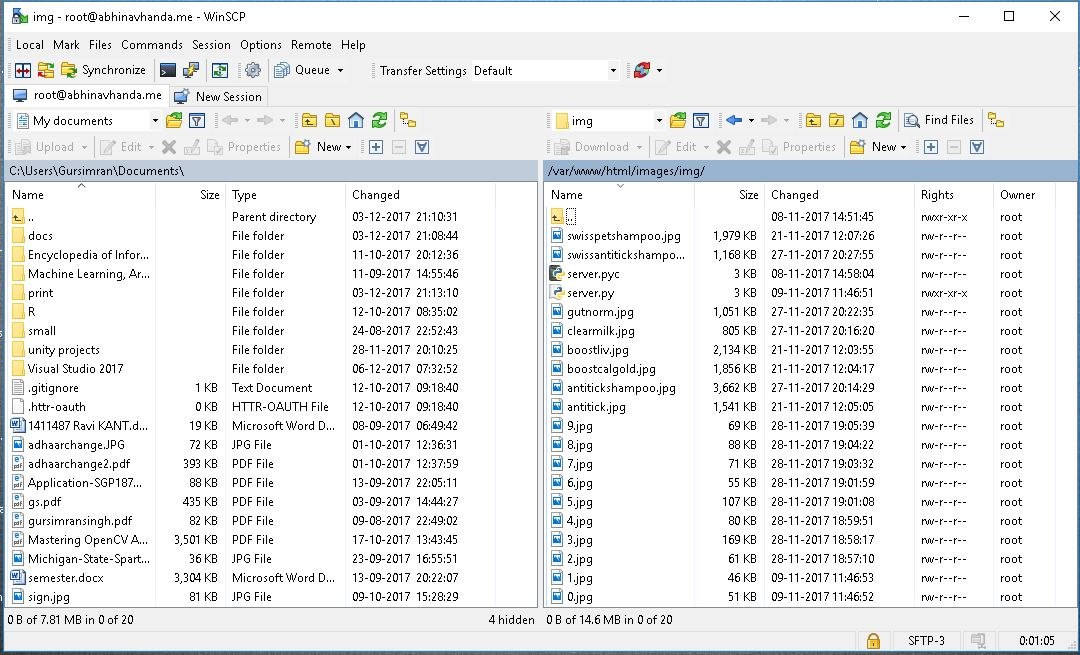
\includegraphics[scale=0.50]{images/server1.png}
\caption{digital ocean server to fetch images}
\end{figure}

DigitalOcean, Inc. is an American cloud infrastructure provider[2] headquartered in New York City with data centers worldwide.DigitalOcean provides developers cloud services that help to deploy and scale applications that run simultaneously on multiple computers. As of December 2015, DigitalOcean was the second largest hosting company in the world in terms of web-facing computers.
In 2003, Ben and Moisey Uretsky who had founded ServerStack, a managed hosting business,wanted to create a new product which would combine the web hosting and virtual servers.The Uretskys, having surveyed the cloud hosting market felt that most hosting companies were targeting enterprise client leaving the entrepreneurial software developers market underserved.In 2011 the Uretskys founded DigitalOcean, a company which would provide server provisioning and cloud hosting for software developers.

In 2012 the Uretskys met co-founder Mitch Wainer following Wainer's response to a Craigslist job listing.The company launched their beta product in January 2012.By mid-2012, the founding team consisted of Ben Uretsky, Moisey Uretsky, Mitch Wainer, Jeff Carr, and Alec Hartman. After DigitalOcean was accepted into TechStars 2012's startup accelerator in Boulder, Colorado, the founders moved to Boulder to work on the product.[11] By the end of the accelerator program[when?], the company had signed up 400 customers and launched around 10,000 cloud server instances.


On January 15, 2013, DigitalOcean became one of the first cloud-hosting companies to offer SSD-based virtual machines. Following a TechCrunch,review which was syndicated by Hacker News, DigitalOcean saw a rapid increase in customers.In December 2013, DigitalOcean opened its first European data center located in Amsterdam.By the end of December 2013, Netcraft reported that DigitalOcean was the fastest growing cloud hosting service in the world in terms of web-facing computer count.During 2014, the company continued its expansion, opening new data centers in Singapore and London.By May 2015, DigitalOcean became the second largest hosting provider in the world according to a report by Netcraft.During 2015 Digita expanded further with a data center in Toronto, Canada.Later in 2016 they continued expansion to Bangalore, India.]As of July 2017, the company has 12 data centers in various parts of the globe.




\begin{figure}[ht]
\centering
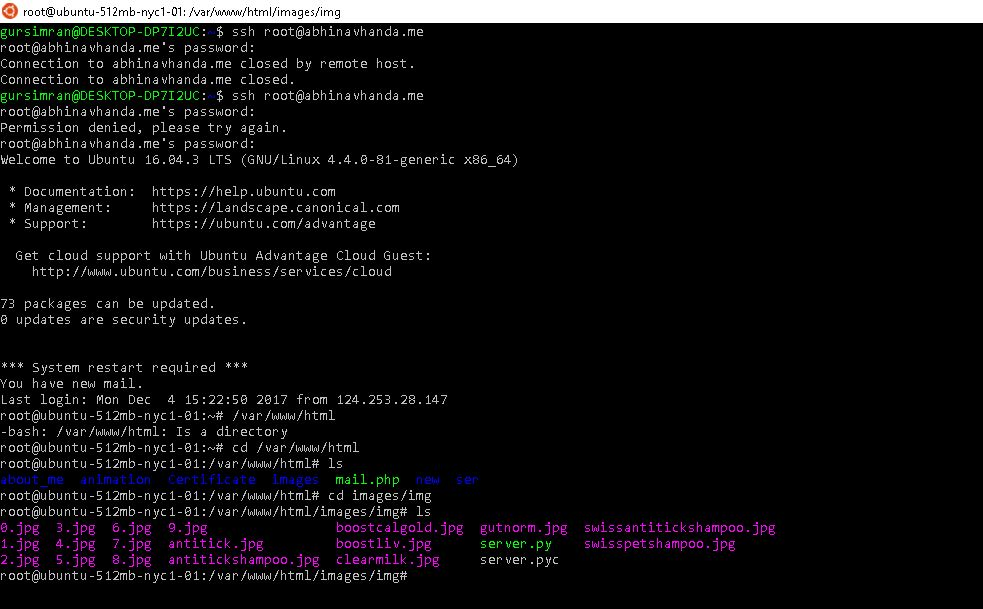
\includegraphics[scale=0.40]{images/server.png}
\caption{digital ocean server Console}
\end{figure}

\subsection{Database Connection Controls and Strings}

\begin{figure}[ht]
\centering
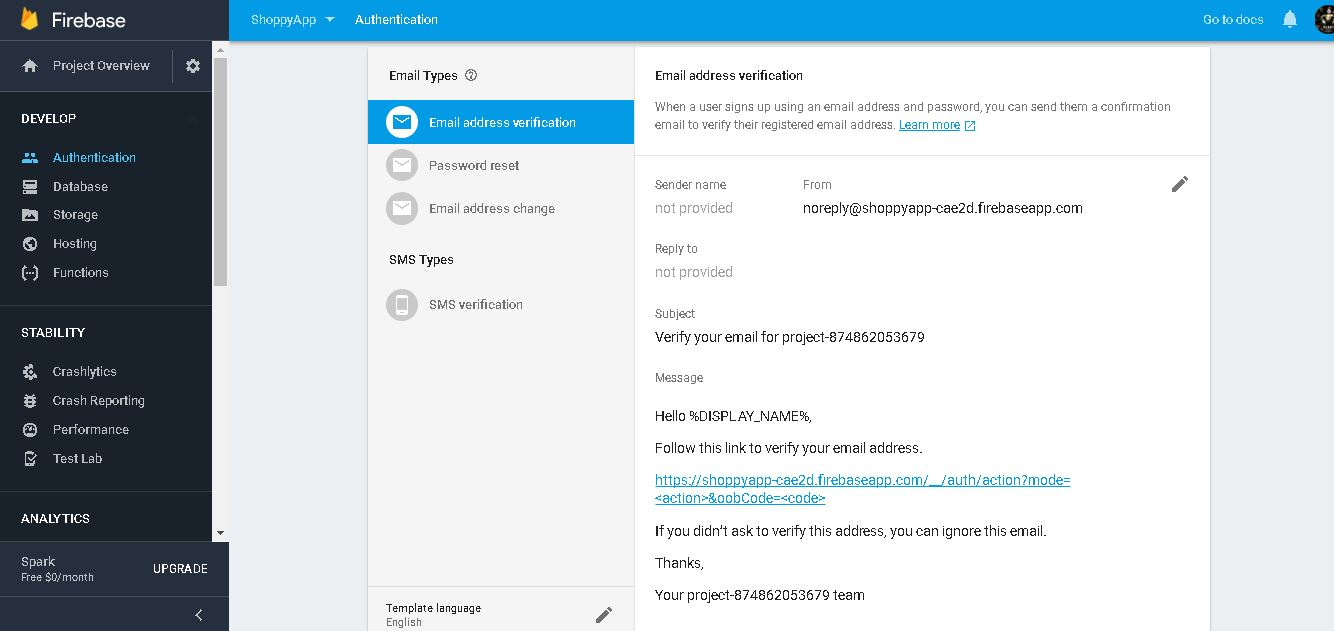
\includegraphics[scale=0.40]{images/firbase14.png}
\caption{Firebase Authentication}
\end{figure}


\begin{figure}[ht]
\centering
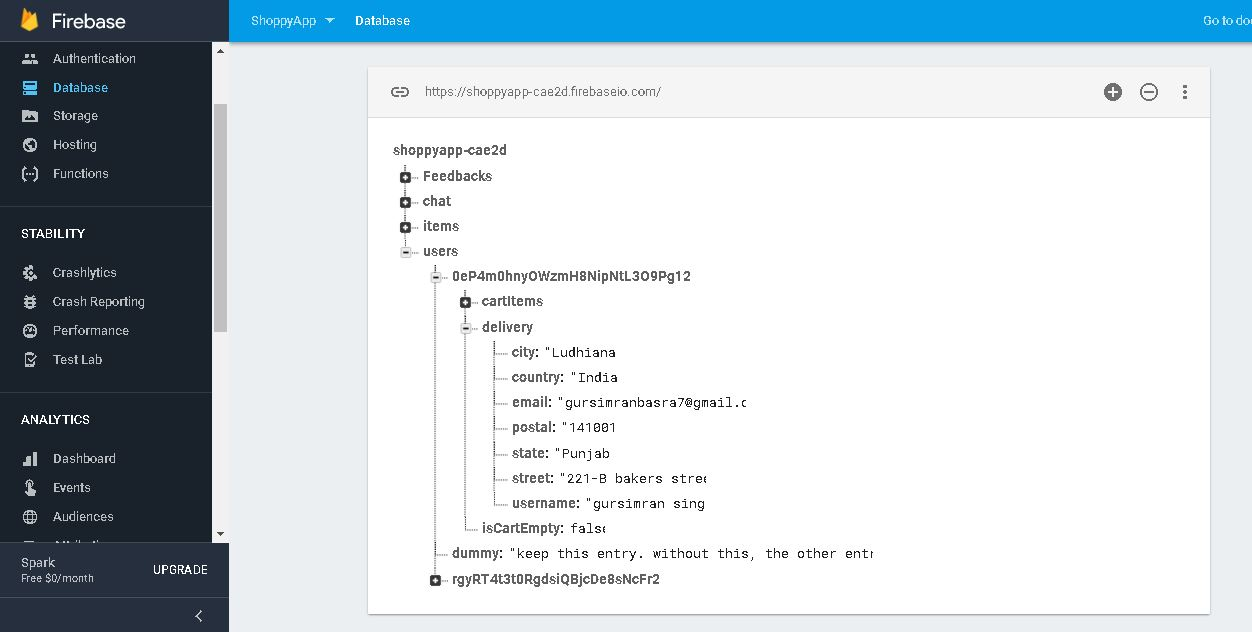
\includegraphics[scale=0.40]{images/Firebase12.png}
\caption{Firebase Database}
\end{figure}

\subsection{Methodology}
Database design methodology provided in this Topic is based on the guideline proposed by Connolly and Begg (2005). They have introduced three main phases of database design methodology, namely: conceptual, logical and physical database design. In this section we provide a description of what a design methodology is, and give a brief overview of the these three main phases of database design.

Design methodology is an approach taken in designing or building things and it serves as a guideline on how things are done. Normally a design methodology is broken down into phases or stages and for each phase the detailed steps are outlined, and appropriate tools and techniques are specified. A design methodology is able to support and facilitate designers in planning, modeling,and managing a database development project in a structured and systematic manner. Validation is one of the key aspects in the design methodology as it helps to ensure that the produced models accurately represent the user
requirement specifications.As mentioned earlier, we are going to adopt the database design methodology proposed by Connolly and Begg for our discussion in this Topic. The methodology consists of three main phases, starting with conceptual, then logical and lastly the physical database design phase. The conceptual database design is aimed to produce a conceptual representation of the required database. The core activity in this phase involves the use of ER modelling in which the entities,relationship and attributes are defined. For the logical design phase, the aim is to map the conceptual model which is represented by the ER model to the logical structure of the database. Among the activities involved in this phase is the use of normalisation process to derive and validate relations. In the physical design phase, the emphasis is to translate the logical structure to the physical implementation of the database using the defined database manangement
system.Besides the above three main phases, this methodology has also outlined eight core steps. The Step 1 is focused on the conceptual database design phase, the Step 2 is focused on the logical database design phase, and the Step 3 to Step 8 are focused on the physical database design phase.  






















































